% -*- root: ../../main.tex -*- %

\section{Design decisions} % (fold)
\label{sec:design_decisions}
  - GDVSEPC
    - why?
  - wf engine partially in wf container
  - ruby / ruby on rails for readability and because i know it, easy to build restful APIs
    - drawback: speed, runtime

  - extra validator
    - defeats purpose of not sending data in gdvsepc but, just POC

  - for sake of simplicity:
    - no compiled language

  - activity types

  - export request synchronous
% section design_decisions (end)

\section{Execution Images} % (fold)
\label{sec:execution_images}

  \subsection{Workflow Image} % (fold)
  \label{sub:workflow_container}
    - application
      - process instance
      - process definition
      - activity instance
      - file helper
      - configuration

  % subsection workflow_container (end)

  \subsection{Activity Image} % (fold)
  \label{sub:activity_containers}
    - application
      - configuration
      - file helper

    - application wrapper
    - manual input wrapper
    - custom code wrapper
  % subsection activity_containers (end)
% section execution_images (end)

\section{System Components} % (fold)
\label{sec:components_implementation}
  \subsection{Workflow Definition Service} % (fold)
    \label{sub:workflow_definition_service}

      \subsubsection{Technical Realization} % (fold)
      \label{ssub:technical_realization}
        The workflow definition service is composed of three components: a Ruby on Rails application which is configured to expose a JSON API, a PostgreSQL database and a data volume container for persistent storage for that database.

        PostgreSQL was chosen as database solution for the definition service, because it supports both relational data, which is useful for storing the workflow, its elements and their relations, and the document-store-like JSONB format, which allows the schema-less storage of configuration information.
        - useful for queryable conf with dynamic structure
        In order to keep the stored data during container restarts or migrations across nodes, the database makes use of a data volume container which provides its working directory.
      % subsubsection technical_realization (end)


      - application
        - ruby on rails (api)
        - components
          - app logic
            - dockerhelper
            - image builder
            - image manager
          - controllers
          - models
            - activity
            - control-flow
            - process-definition
            - workflow
          - serializers
            - process definition image serializer
            - workflow full serializer

      - database
        - postgresql
      - data volume
        - docker volume

    \begin{figure}[htbp]
      \centering

      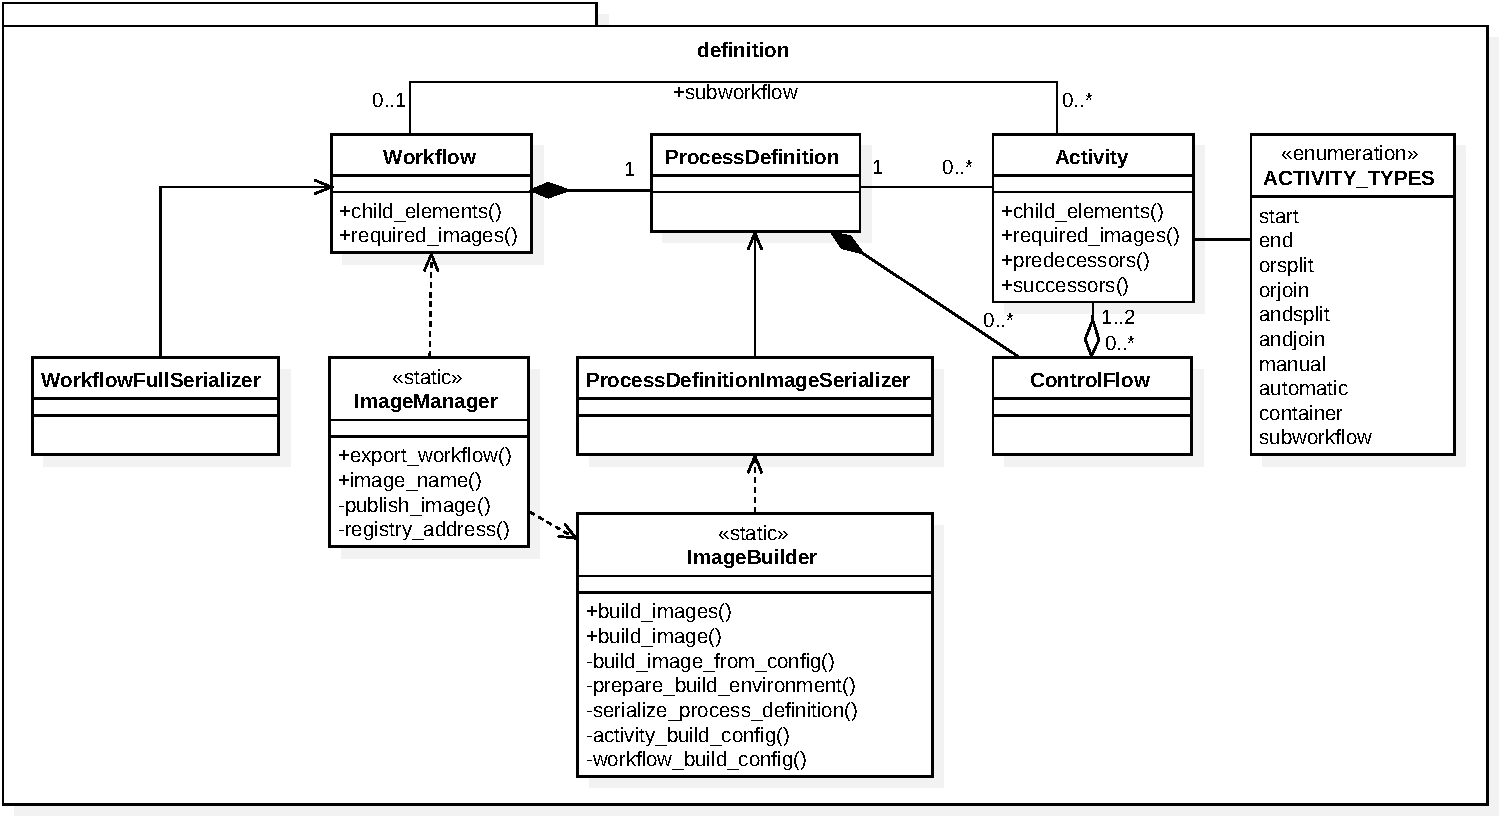
\includegraphics[width=0.95\textwidth]{content/images/class_diagram_definition-crop.pdf}
      \caption*{\scriptsize Controllers omitted for the sake of simplicity. Workflow, ProcessDefinition, Activity and ControlFlow each have a controller with the respective pluralized name plus a `Controller' suffix.}
      \caption{UML Class Diagram for the Definition Service}
      \label{fig:label}
    \end{figure}


    \subsubsection{Exporting a Workflow} % (fold)
      \label{ssub:exporting_a_workflow}
      If the user requests the export of a workflow, the request is forwarded to the \texttt{ImageManager}.
      In order to export a workflow, the first step is to identify all of its elements that require to be wrapped in an image. Obviously, one of them is the workflow itself. The other required images are determined by traversing the workflow's process definition recursively. Each activity has to be exported, too, and each sub-workflow has a method that exposes the Docker images it requires beyond that. It does so by passing the call for required images on to the referenced workflow, which collects its required images analogously, and returning the result.

      The \texttt{ImageBuilder} then iterates over all these elements and creates a correspondent image for each. Starting with the respective base image, it creates the files which are specific to the current element from the activity's or workflow's configuration, \ie the input/output validation schemata, the element's description file, and in case of a workflow the process definition, in a temporary directory . The \texttt{ImageBuilder} then copies these files to the image and names it after the workflow element that it represents.

      The \texttt{ImageManager} then uploads all images which were successfully built to the private repository and publishes a notification of the successful build via the message broker.
      % subsubsection exporting_a_workflow (end)
    % subsection workflow_definition_service (end)

  \subsection{Organization Management Service} % (fold)
    \label{sub:organization_management_service}
      - application
        - controllers
        - models
          - role
            - ancestors
          - user
            - with role
      - database
        - postgresql
      - data volume
        - docker volume
    % subsection organization_management_service (end)

  \subsection{Worklist Service} % (fold)
    \label{sub:worklist_service}
      - application
        - controllers
        - models
          - worklist item
      - database
        - postgresql
      - data volume
        - docker volume
    % subsection worklist_service (end)

  \subsection{Workflow Engine Service} % (fold)
    \label{sub:workflow_engine_service}
      - application
    % subsection workflow_engine_service (end)

  \subsection{Developer Gateway} % (fold)
    \label{sub:developer_gateway}
      - application
        - backend: rails
        - frontend: angular app
    % subsection developer_gateway (end)

  \subsection{User Gateway} % (fold)
    \label{sub:user_gateway}
      - application
        - backend: rails
        - frontend: angular app
    % subsection user_gateway (end)

  \subsection{Message Oriented Middleware} % (fold)
    \label{sub:message_oriented_middleware}
      For this prototype, RabbitMQ was chosen as message oriented middleware, because it is well documented and has various ruby clients, \eg \emph{Hutch} and \emph{Bunny}.

      RabbitMQ exists as a pre-configured Docker image on the Docker Hub and can thus be utilized easily. The configuration of RabbitMQ in this image takes place when the respective container is run, which allows its configuration in the \texttt{docker-compose} configuration file.
      For the sake of simplicity, no authentication mechanism was introduced besides the simple default username/password combination.
    % subsection message_oriented_middleware (end)

  \subsection{Infrastructure Management Service} % (fold)
    \label{sub:infrastructure_management_service}
      - application
        - app logic
          - docker helper
          - environment manager
        - controllers
          - servers controller
        - models
          - server

    % subsection infrastructure_management_service (end)

  \subsection{Registry} % (fold)
    \label{sub:registry}
    % subsection registry (end)

  \subsection{Provisioning Service} % (fold)
    \label{sub:provisioning_service}
      - application
    % subsection provisioning_service (end)
% section components (end)


\begin{figure}[htbp]
  \centering
  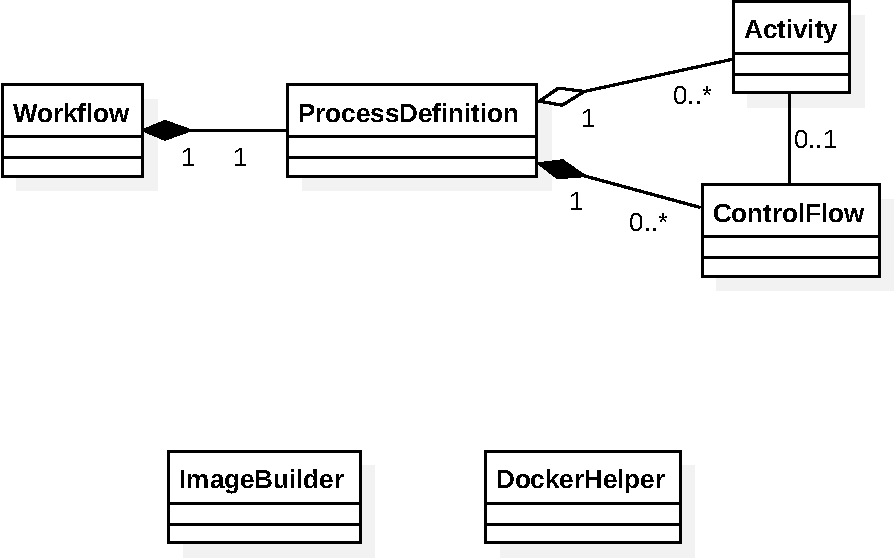
\includegraphics[width=0.95\textwidth]{content/images/class_d_definition-crop.pdf}
  \caption{UML Class Diagram for Workflowe Definition Service}
  \label{fig:uml_class_diagram_definition_service}
\end{figure}

\section{Implementation Issues} % (fold)
\label{sec:implementation_issues}

% section implementation_issues (end)
